\chapter{Materiais e Métodos}\label{cap:metodologia}

Este capítulo descreverá todo o processo para a criação da metodologia usada.
Desde a descrição e adaptação do conjunto de dados utilizado, cobrindo as escolhas dos modelos de classificação até a forma de avaliação dos resultados,
além das tecnologias utilizadas em cada passo.

Apesar de ser possível classificar a situação de alagamento de uma rua em diferentes níveis, para o problema de classificação descrito,
as diferentes situações foram simplificadas para um problema binário, onde o objetivo é definir se a quantidade de água na rua permite o trânsito de veículos normalmente (classe 0),
ou se a quantidade é suficiente para impactar o trânsito (classe 1).

\section{Conjunto de dados}\label{sec:dataset}

O conjunto de dados consiste em imagens de 77 câmeras diferentes da cidade do Rio de Janeiro, capturadas pelo sistema de câmeras do \Acrfull{cor}.
Neste conjunto, cada câmera possui 30 imagens para cada uma das classes deste problema de classificação binário.
Ou seja, o conjunto de dados é formado por 60 imagens de cada câmera, totalizando 4.620 imagens.
Do total de 77 câmeras, 60 foram escolhidas para compor o conjunto de treino e 17 câmeras para validação, ou seja, 78\% das câmeras compõem o conjunto de treino e 22\% o conjunto de validação.

Este trabalho frequentemente se refere ao conjunto de dados usado pelo número de câmeras, em vez de descrever diretamente o número de imagens.
Isso é feito propositalmente, visto que foi decidido não utilizar imagens da mesma câmera em treino e em validação, para evitar qualquer tipo de viés em sua validação.
Portanto, cada câmera do conjunto de dados pertence somente ao conjunto de treino ou ao conjunto de validação.

Como as imagens foram capturadas em uma cidade movimentada durante o período de chuvas, uma variedade de imagens foi utilizada para o treinamento,
desde ruas vazias em um dia ensolarado até tráfego intenso em dias chuvosos durante a noite.
Devido a chuvas extremamente fortes, algumas lentes de câmeras estavam muito molhadas para distinguir o que era exibido. Essas imagens não foram incluídas no conjunto de dados.

Ao longo do ano, foram captadas imagens de 472 câmeras distintas, com diferentes proporções de imagens de cada classe para cada câmera.
Dessa forma, para criar um conjunto de dados balanceado,
foram escolhidas as câmeras com quantidade suficiente de imagens de ambas as classes para que todas as câmeras do conjunto de dados tenham a mesma quantidade de imagens.

% -----------------------

\subsection{Captação de imagens}
As imagens foram captadas ao longo de 2023 em diferentes condições de iluminação e em diferentes épocas de chuva, com variadas intensidades pluviométricas.
Foi necessário captar tais imagens de maneira eficiente e inteligente, visto que o sistema de câmeras do \acrshort{cor} é composto por milhares de câmeras,
tornando custoso o monitoramento de todas elas, além de as chuvas, apesar de intensas, serem imprevisíveis — podendo ocorrer a qualquer hora e com durações bastante variadas.

O sistema de captação foi desenvolvido em Python \cite{van1995python}, utilizando a API do Waze para receber notificações de possíveis situações de alagamento.
A biblioteca OpenCV \cite{itseez2015opencv} foi utilizada para a captura das imagens, e a API do Google Cloud, para upload e armazenamento.
Foram utilizados alertas do aplicativo Waze sobre alagamento de ruas e notificações do próprio sistema do \acrshort{cor} para definir quais ruas da cidade do Rio de Janeiro estavam alagadas e, assim, iniciar a captação de imagens dessas ruas.

% -----------------------
\subsection{Análise de imagens}
Para a classificação das imagens, foi criada uma aplicação web baseada em Flask e utilizando MongoDB como banco de dados.
As imagens já estavam separadas em seis (6) níveis definidos pelo próprio \acrshort{cor}. Estes níveis, em ordem crescente de severidade, são: Normal; Poça; Lâmina; Alagamento; Transbordo; e Bolsão.

Para simplificar, tendo em vista que não há um limite claramente definido entre cada uma dessas classificações, as classes 'Normal' e 'Poça' foram definidas como classe 0,
visto que não há impacto no trânsito de veículos. A partir do surgimento de lâminas d'água,
o trânsito de veículos começa a ser afetado, visto que estes devem diminuir sua velocidade para evitar derrapagem \cite{michelinaquaplaning}.
Então, a partir do nível 3, 'Lâmina', as classes mais severas foram definidas como classe 1.

A Figura \ref{fig:class0_1} mostra uma importante avenida na Zona Sul do Rio de Janeiro, no entorno da Lagoa Rodrigo de Freitas:
a Av. Epitácio Pessoa, na altura da Rua Maria Quitéria, no lado desta lagoa próximo ao bairro de Ipanema.
A Figura \ref{fig:class0_2} mostra a Rua Jardim Botânico, no cruzamento com a Rua Pacheco Leão, no bairro Jardim Botânico.
Estas figuras são exemplos de vias classificadas como \textbf{não alagadas}, ou classe 0.
Quando há água na via, mas ela não impede o tráfego de veículos, decidiu-se que tais situações não seriam classificadas como \textit{alagamento}.

\begin{figure}[htb]
\centerline{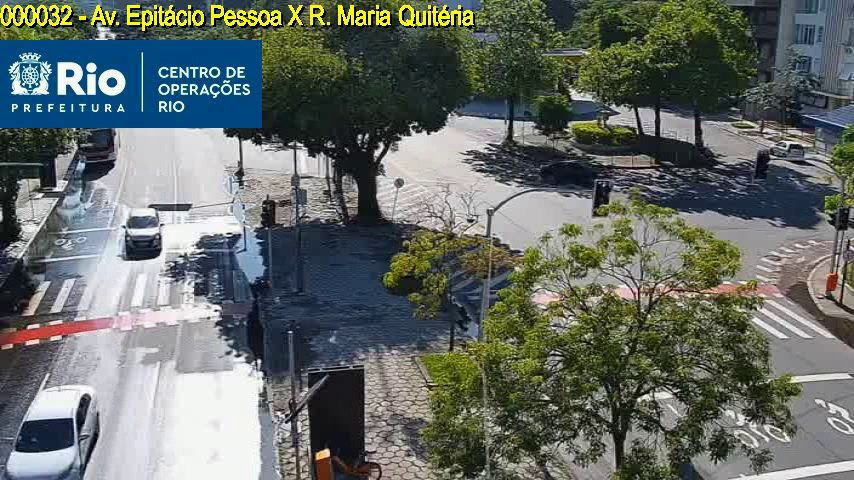
\includegraphics[width=0.8\linewidth]{images/0/CODE32 2023-02-22 08-15-04-6.jpg}}
\caption{Via completamente seca, rotulada como classe 0}
\label{fig:class0_1}
\end{figure}

\begin{figure}[htb]
\centerline{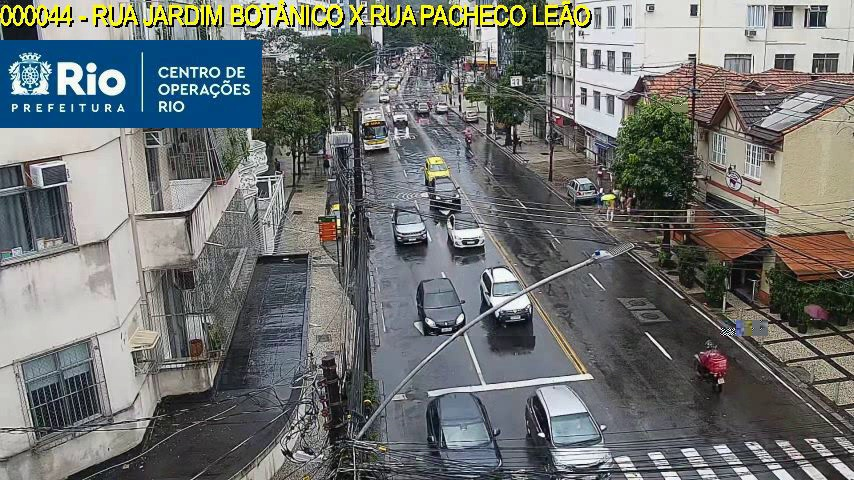
\includegraphics[width=0.8\linewidth]{images/0/CODE44 2023-08-20 13-30-31-6.jpg}}
\caption{Rua molhada, ainda rotulada como classe 0}
\label{fig:class0_2}
\end{figure}

Por outro lado, a Fig. \ref{fig:class1_1} e a Fig. \ref{fig:class1_2} mostram capturas de vias classificadas como \textbf{alagadas}, ou classe 1.
Em ambas as imagens, é possível observar água cobrindo grande parte da via, dificultando ou até impossibilitando a passagem de veículos.
A Fig. \ref{fig:class1_1} apresenta o exemplo de uma rua localizada na zona norte da cidade, parcialmente alagada, onde o trânsito de veículos é dificultado, embora as calçadas ainda possam ser identificadas.
Por sua vez, a Fig. \ref{fig:class1_2} mostra o exemplo de uma rua na Zona Sul, onde não há distinção visual entre calçada e via, ambas completamente submersas.
Essas situações constituem a classe \textit{alagamento}.

\begin{figure}[htb]
\centerline{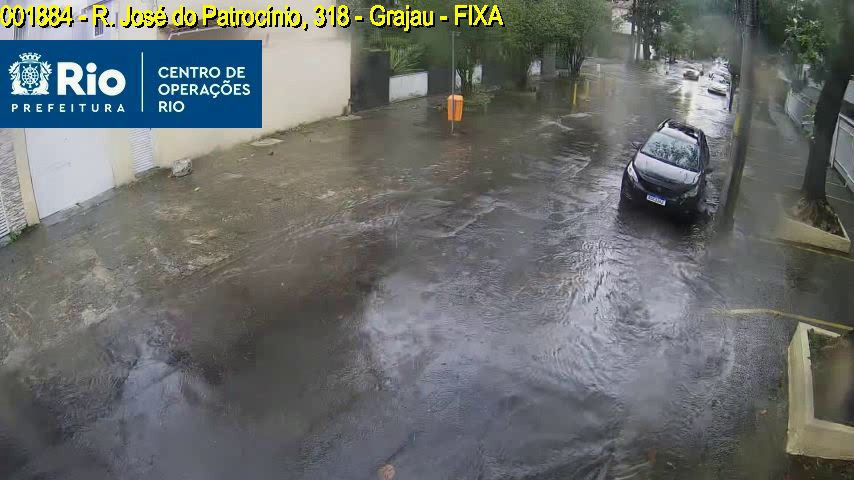
\includegraphics[width=0.8\linewidth]{images/1/CODE1884 2023-08-20 12-56-29-9.jpg}}
\caption{Rua parcialmente alagada (classe 1).}
\label{fig:class1_1}
\end{figure}

\begin{figure}[htb]
\centerline{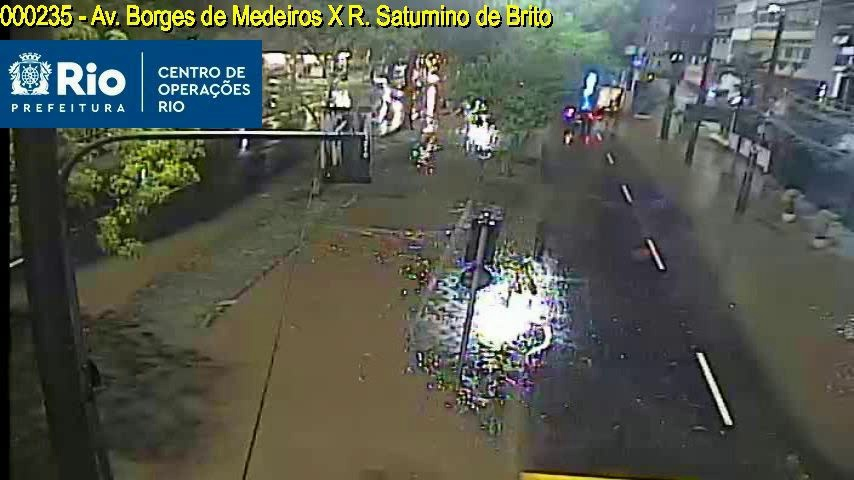
\includegraphics[width=0.8\linewidth]{images/1/CODE235 2023-02-07 20-11-08-9.jpg}}
\caption{Avenida totalmente alagada (classe 1).}
\label{fig:class1_2}
\end{figure}

As Figuras \ref{fig:class0count} e \ref{fig:class1count} apresentam, respectivamente, a quantidade de imagens da classe 0 e da classe 1 (eixo vertical) para cada câmera (eixo horizontal).
A Figura \ref{fig:totalcount} exibe a distribuição total de imagens por câmera, considerando ambas as classes conjuntamente.

Devido à grande quantidade de câmeras, seus identificadores (ou códigos) não são exibidos no eixo horizontal dessas figuras.
Entretanto, a Tabela apresentada no Apêndice \ref{apendA} relaciona o identificador de cada câmera e sua respectiva quantidade de imagens para cada classe.

Essas figuras representam o conjunto de dados original, composto por imagens capturadas de 472 câmeras do sistema do \acrshort{cor}, sem qualquer balanceamento prévio entre as classes.
Nas figuras, a correspondência entre as classes (\textbf{alagadas} ou \textbf{não alagadas}) e as cores (azul e vermelho) é utilizada para distinguir visualmente a quantidade de imagens de cada classe associada a cada câmera, conforme as barras representadas no eixo horizontal dos histogramas de distribuição.

Observa-se que algumas câmeras possuem significativamente mais imagens da classe 1 (alagadas) do que outras, possivelmente em decorrência da maior incidência de chuvas nas regiões onde essas câmeras estão instaladas.
Dessa forma, a utilização desse conjunto de dados, sem uma análise criteriosa da representatividade de cada câmera, poderia introduzir viés no treinamento dos modelos, comprometendo a capacidade de generalização dos mesmos.
\begin{figure}[htb]
    \centerline{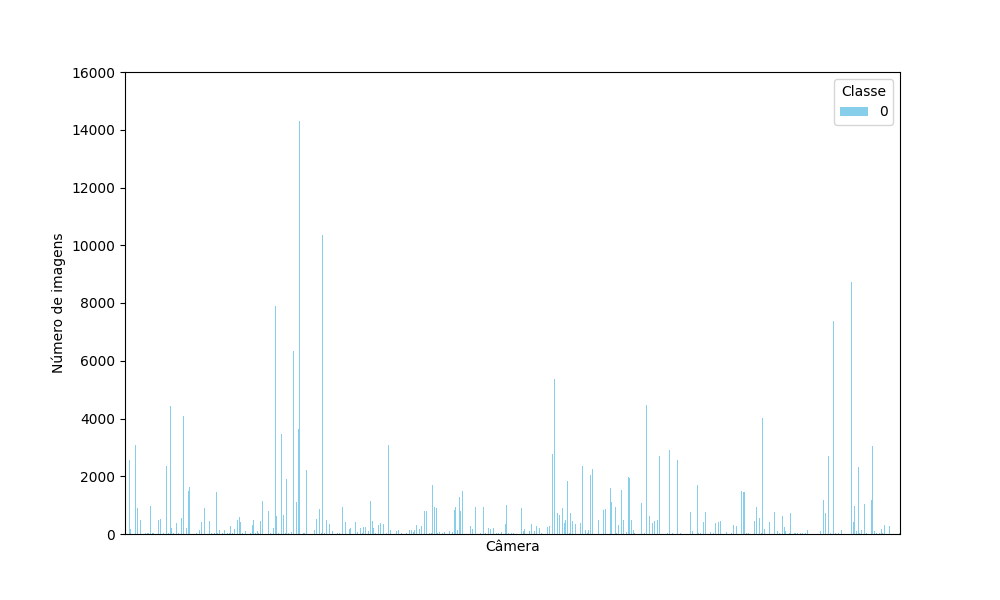
\includegraphics[width=1\linewidth]{images/metodologia/class_0_count_code.png}}
    \caption{Quantidade de imagens de normalidade por câmera disponível.}
    \label{fig:class0count}
\end{figure}

\begin{figure}[htb]
    \centerline{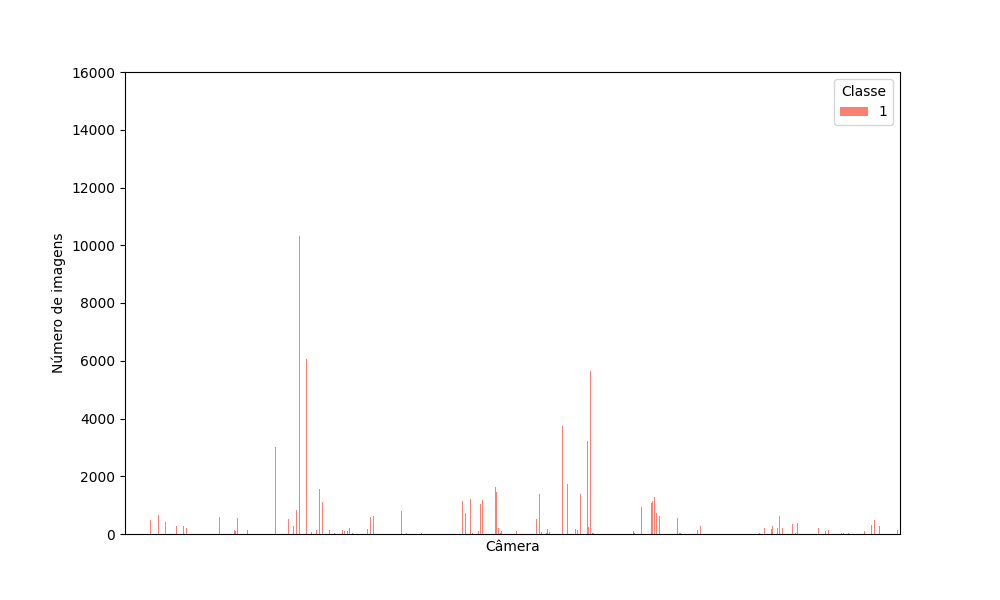
\includegraphics[width=1\linewidth]{images/metodologia/class_1_count_code.png}}
    \caption{Quantidade de imagens de alagamento por câmera disponível.}
    \label{fig:class1count}
\end{figure}

\begin{figure}[htb]
    \centerline{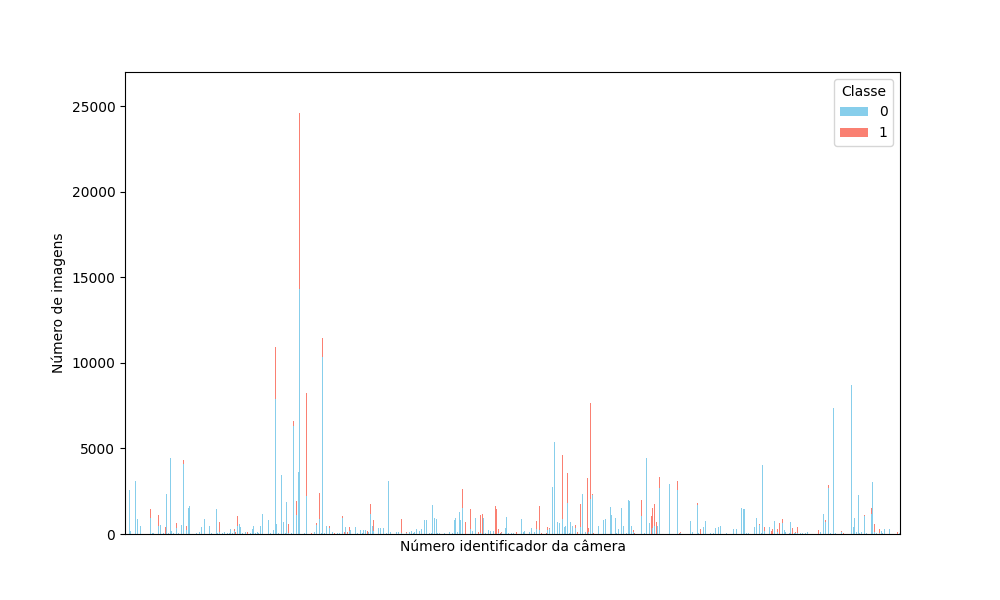
\includegraphics[width=1\linewidth]{images/totalcount_code.png}}
    \caption{Quantidade de imagens de cada classe por câmera disponível.}
    \label{fig:totalcount}
\end{figure}

A Figura \ref{fig:histcodes} mostra uma distribuição de frequência de câmeras por quantidade de imagens, separadas em intervalos de 100 imagens.
O intervalo com maior ocorrência de câmeras indica o desbalanceamento do conjunto de imagens captadas onde 206 câmeras, ou 43,6\%, possuem até 100 imagens ao todo. 

\begin{figure}[htb]
    \centerline{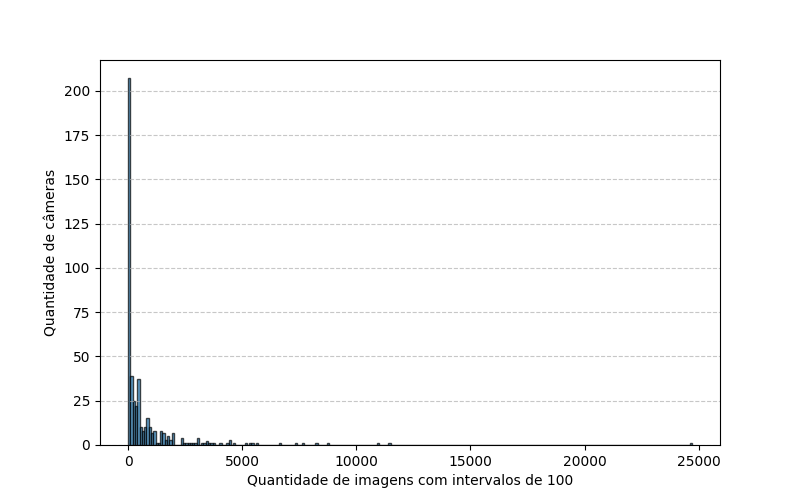
\includegraphics[width=1\linewidth]{images/metodologia/histcodes.png}}
    \caption{Histograma de quantidade de imagens de alagamento por câmera disponível.}
    \label{fig:histcodes}
\end{figure}

A Figura \ref{fig:histcodes} apresenta a distribuição de frequência das câmeras em função da quantidade total de imagens, agrupadas em intervalos de 100 imagens.
Observa-se que o intervalo com maior frequência concentra as câmeras que possuem até 100 imagens no total, independentemente da classe.
Este dado evidencia de forma clara o desbalanceamento do conjunto de dados, uma vez que 206 câmeras (o que representa aproximadamente 43,6\% do total) encontram-se nesse intervalo.

Tal distribuição reforça a necessidade de um criterioso processo de seleção e balanceamento das câmeras que compõem o conjunto final utilizado para treinamento e validação dos modelos.
Caso contrário, o treinamento sobre este conjunto poderia sofrer impacto negativo, levando à criação de modelos enviesados, com baixa capacidade de generalização, sobretudo para situações observadas em câmeras com menor representatividade no conjunto de dados original.

\begin{figure}[htb]
\centerline{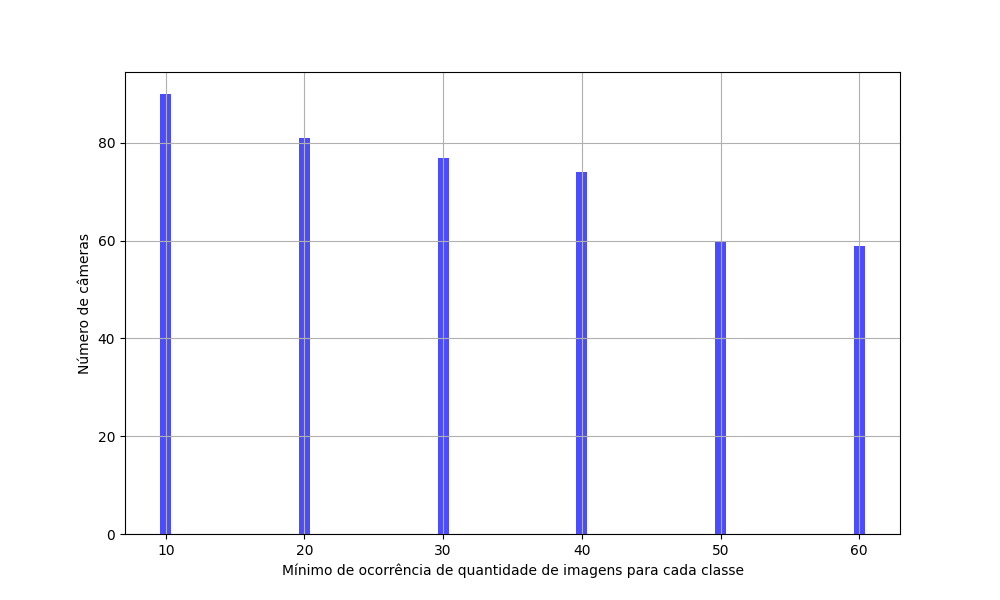
\includegraphics[width=1\linewidth]{images/balancedcodes.png}}
\caption{Quantidade de câmeras com um número mínimo de imagens de cada classe.}
\label{fig:balancedcodes}
\end{figure}

Portanto, as arquiteturas de redes neurais convolucionais foram treinadas utilizando um conjunto de dados composto por 77 câmeras, totalizando 4620 imagens. Esse conjunto foi cuidadosamente balanceado, contendo 30 imagens de cada classe para cada câmera — ou seja, 60 imagens por câmera. A divisão dos dados considerou 60 câmeras destinadas ao treinamento e 17 câmeras para validação, correspondendo, respectivamente, a aproximadamente 78\% e 22\% do total de câmeras.

Adicionalmente, o conjunto de dados excedente — composto pelas câmeras e imagens que não foram selecionadas para os conjuntos de treinamento e validação — foi utilizado para a criação de um conjunto de teste. Esse conjunto de teste foi construído por meio da seleção aleatória de 150 imagens de cada classe, totalizando 300 imagens. Diferentemente do critério adotado para treinamento e validação, na formação do conjunto de teste não houve restrição quanto à representação equitativa de cada câmera, visto que seu objetivo principal é avaliar a capacidade de generalização dos modelos para dados não vistos e com maior variabilidade.

Com isso, o conjunto de dados completo utilizado neste trabalho é composto por 4920 imagens, sendo 4620 destinadas ao treinamento e validação e 300 reservadas para teste.

Por fim, após a primeira etapa de avaliação dos modelos baseados em \acrshort{cnn}s, foi realizada uma reanálise da quantidade de imagens por câmera, visando avaliar se diferentes quantidades de imagens poderiam impactar significativamente os índices de desempenho dos modelos — tais como acurácia, precisão, revocação e F1-Score. Esse estudo adicional é detalhado na Seção \ref{sec:cameraquantity}, onde são discutidos os impactos da variação na quantidade de imagens por câmera sobre o desempenho dos modelos.
% -----------------------
\subsection{Pré Processamento}\label{subsec:datapreprocessing}

Diversas etapas de pré-processamento foram aplicadas com o objetivo de melhorar a qualidade das imagens e, consequentemente, a capacidade de generalização dos modelos de aprendizado de máquina.

Inicialmente, uma máscara foi aplicada sobre todas as imagens do conjunto de dados para remover o logotipo institucional do \acrshort{cor}, localizado na região superior esquerda. Este logotipo consiste no brasão da cidade do Rio de Janeiro, acompanhado de texto em branco sobre um fundo azul. A remoção dessa informação visual foi considerada essencial, uma vez que sua presença constante poderia introduzir um viés indesejado no processo de aprendizado, levando o modelo a associar características do logotipo às classes de alagamento, comprometendo sua capacidade de generalização.

A estratégia adotada para essa remoção consistiu na aplicação de uma máscara de preenchimento nulo (valores de pixel zerados) sobre a região específica ocupada pelo logotipo. Tal abordagem foi viável devido à posição fixa e invariante desse elemento em todas as imagens. No entanto, não foi possível realizar uma reconstrução semântica ou interpolação da região ocultada, uma vez que não existiam quadros de referência sem a presença do logotipo no dataset original.

Em uma segunda etapa, buscou-se corrigir problemas relacionados à exposição excessiva presentes em parte das imagens, especialmente aquelas capturadas sob condições de elevada luminosidade. Para isso, foi realizada a conversão do espaço de cor original, do modelo RGB para o espaço de cor $YC_rC_b$. Esta conversão foi escolhida porque isola o componente de luminância (canal $Y$) dos componentes cromáticos ($C_r$ e $C_b$), permitindo intervenções específicas na intensidade da claridade da imagem sem afetar suas características de cor.

O ajuste da claridade foi realizado através de uma transformação linear aplicada exclusivamente sobre o canal de luminância ($Y$), segundo a seguinte equação:

\begin{equation}
    \label{eqn:fb}
    Y' = FC \cdot Y
\end{equation}

onde $FC$ representa o Fator de Claridade, um escalar real positivo no intervalo $(0, 1]$. Este fator controla a intensidade da redução da luminosidade. Na fase inicial dos experimentos, adotou-se $FC = 0,5$ como valor de referência, com o objetivo de reduzir a claridade à metade. Valores distintos para $FC$ foram posteriormente analisados na Seção \ref{sec:bestmodel}, buscando otimizar o desempenho do modelo.

Após a aplicação do fator de claridade, as imagens foram reconvertidas do espaço $YC_rC_b$ para RGB, garantindo que pudessem ser visualizadas e processadas de acordo com os padrões dos modelos de \acrshort{cnn} utilizados.

As Figuras \ref{fig:samplebright} e \ref{fig:samplebright_half} ilustram o efeito visual da aplicação do fator de claridade. A primeira apresenta a imagem na condição original, enquanto a segunda demonstra a mesma cena após a aplicação de $FC = 0,5$. É possível observar uma significativa redução na intensidade de claridade, preservando, contudo, a integridade das informações cromáticas e estruturais relevantes para a tarefa de classificação.

\begin{figure}[htb]
    \centerline{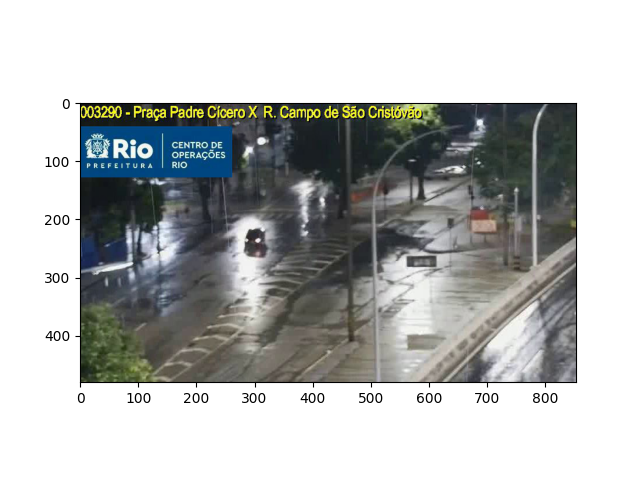
\includegraphics[width=1\linewidth]{images/metodologia/samplebright.png}}
    \caption{Exemplo de região sem alteração no canal \textit{Y}.}
    \label{fig:samplebright}
\end{figure}
\begin{figure}[htb]
    \centerline{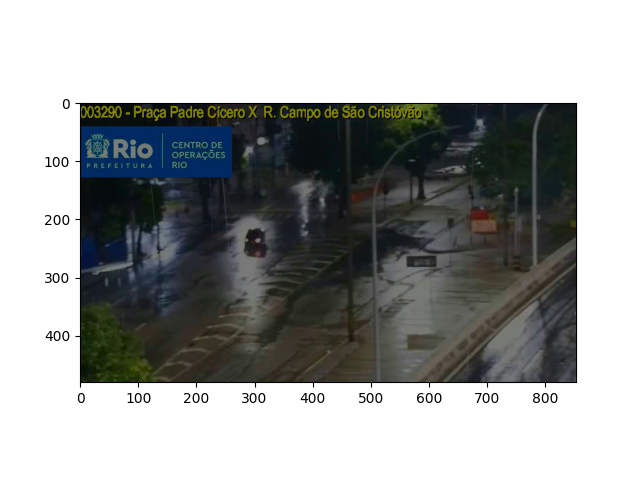
\includegraphics[width=1\linewidth]{images/metodologia/samplebright_half.png}}
    \caption{Exemplo de mesma região com 50\% do valor original de \textit{Y}.}
    \label{fig:samplebright_half}
\end{figure}

Para introduzir mais variedade às imagens no treinamento, em seguida foi aplicada uma inversão horizontal aleatória com uma probabilidade de 50\% nos dados de entrada.
Em outras palavras, cada imagem da divisão de treinamento tem 50\% de chance de ser invertida horizontalmente ou não.

Além disso, transformações padrão de redimensionamento, corte e normalização de intensidades são usadas para preparar as imagens para cada modelo \textit{CNN}.
É aplicado aos dados, inicialmente, um processo de redimensionamento para transformar cada quadro, ajustando-o ao tamanho esperado de cada modelo,
onde as imagens com dimensão 854 x 480 pixels são redimensionadas para 256 x 256 pixels.
Então, elas são submetidas a um corte de dimensão 224 x 224 pixels, com o mesmo centro da imagem.
Com exceção do \textit{Inception}, que redimensiona para 342 x 342 pixels e realiza um corte central de 299 x 299 pixels.
Os valores do conteúdo de cada pixel são redimensionados para estarem no intervalo [0,1].

Finalmente, todo o conjunto de dados foi normalizado pela média e desvio padrão específicos de cada modelo:
todos os modelos avaliados têm a mesma matriz média de (0,485; 0,456; 0,406) e matriz de desvio padrão de (0,229; 0,224; 0,225) para cada canal $RGB$, usados para normalizar a imagem.% ----------------------------------------------------------

\section{Modelos de classificação}\label{sec:methodology_models}

Com base na nos trabalhos da literatura sobre alagamento urbano anteriormente apresentados, os modelos MobileNetV2 \cite{mobilenetv2}, VGG19 \cite{vgg}, InceptionV3 \cite{inception} e DenseNet \cite{densenet} foram avaliados.
Além disso, a arquitetura de \acrfull{vit}\cite{vit} foi incluída. Essa adição foi feita porque vários modelos de classificação de imagens de alto desempenho são baseados em arquiteturas $Visual$ $Transformers$, como $ViT-Huge$ usado no conjunto de dados CIFAR-10 \cite{dosovitskiy2021image} e $ViT-Large$ no conjunto de dados STL-10 \cite{gesmundo2022continual, kabir2023reduction}.

Todos os modelos foram treinados em 50 épocas, onde o \textit{Early Stopping} foi empregado com uma restrição de 10 épocas e decaimento da taxa de aprendizagem de 0,1. Três diferentes taxas de aprendizagem foram aplicadas em todos os modelos, visto que as diferentes complexidades dos modelos podem resultar em diferentes taxas de aprendizagem ótimas. O \acrfull{sgd} foi usado como otimizador inicialmente, entretanto, outros otimizadores foram testados após a avaliações dos modelos, como pode ser visto na seção \ref{sec:optimizer}.

A transferência de aprendizado foi aplicada a todos os modelos, inicializando-os com os pesos padrões do IMAGENET. Isso foi feito para utilizar os pesos aprendidos anteriormente para auxiliar no aprendizado dos pesos das novas classes \cite{kolesnikov2020big}. Posteriormente, a última camada totalmente conectada foi modificada para ter apenas duas saídas, se adequando ao problema de classificação binária.
% ----------------------------------------------------------
\section{Avaliação dos modelos}

Para avaliar o desempenho dos cinco modelos com diferentes taxas de aprendizagem, inicialmente foi utilizada a acurácia para distinguir o melhor modelo.
Após a identificação do melhor modelo, a precisão e a revocação também foram utilizadas para melhor entender seu desempenho.

Como o conjunto de dados está completamente balanceado, conforme mencionado na Seção \ref{sec:dataset}, com ambas as classes igualmente representadas, esses avaliadores fornecem um cenário adequado para a compreensão dos resultados.
Adicionalmente, todas as câmeras possuem o mesmo número de imagens, garantindo, assim, uma representação equilibrada entre as fontes de dados e suas distribuições pela cidade.

Para calcular a acurácia, a precisão e a revocação, inicialmente foram obtidos os seguintes valores:
Verdadeiros Positivos (TP), que correspondem ao número de rótulos positivos classificados corretamente pelo modelo;
Verdadeiros Negativos (TN), que representam os rótulos negativos classificados corretamente;
Falsos Positivos (FP), que são os rótulos negativos classificados incorretamente como positivos;
e Falsos Negativos (FN), que indicam o número de rótulos positivos classificados de forma incorreta como negativos.

O primeiro índice de avaliação selecionado para análise foi a acurácia,
pois ela fornece uma visão geral da capacidade do modelo em classificar corretamente os exemplos em um conjunto de dados balanceado. 

A acurácia pode ser calculada pela seguinte fórmula:
\begin{equation}
    \label{eqn:accuracy}
    Acuracia = \frac{TP+TN}{TP+TN+FP+FN}
\end{equation}

O índice de avaliação de precisão indica a porcentagem de imagens classificadas como positivas que realmente pertencem à classe positiva \cite{FAWCETT2006861}. 
É especialmente relevante para aumentar a confiabilidade do modelo na identificação correta da situação de inundação.

A Equação \ref{eqn:precision} formaliza o cálculo da precisão:
\begin{equation}
    \label{eqn:precision}
    Precisao = \frac{TP}{TP+FP}
\end{equation}

Além disso, a revocação pode ser empregada como um avaliador final para calcular a taxa de imagens positivas classificadas corretamente \cite{MurphyProbabilistic}. 
Ela é útil para garantir que o menor número possível de situações de inundação seja classificado incorretamente. A revocação mede a capacidade do modelo de identificar corretamente todas as instâncias relevantes.
A equação a seguir define o cálculo da revocação:
\begin{equation}
    \label{eqn:recall}
    Revocacao = \frac{TP}{TP+FN}
\end{equation}

O próximo capitulo apresenta os resultados obtidos. 